%LTeX: language=de-DE
\chapter{Forschung und Entwicklung}
    \section{Geschichte}\label{sec:geschichte}
        \textsc{Lawrence E. Daly} reichte 1948 ein Patent zu einem neuartigen Werkstoff ein, der hart, zäh, thermoplastisch verformbar
        und gleichzeitig in kochendem Wasser formbeständig sein soll. Die Idee war, dem damals bereits bekannten Acrylnitril-Styrol-Kopolymer
        das damals ebenfalls bekannte und kommerziell verfügbare 1,3-Butadien \enquote{homogen und untrennbar}
        beizumischen. Als Nebeneffekt wurde das so erhaltene neuartige Material durch die neu hinzugefügte, elastomere Komponente
        deutlich schlagfester (vgl. \cite{ABS.patent.1948.Daly.10191946}).
        \medskip
        Die Synthese des hierzu notwendigen Acrylnitrils war aber aufwendig, teuer und ineffizient. Knapp 10 Jahre später
        reichten \textsc{James D. Idol Jr.} und \textsc{Shaker Heights} für das Unternehmen \textsc{Sohio} ein Patent zu einem verbesserten Verfahren
        der Synthese ein, das als Beiprodukte die damals ebenfalls teuren Stoffe Acrylaldehy und Propensäure abwarf. Mit
        bereits festem Stand in der Erdölindustrie und einem Patent zur effizienten Produktion eines der notwendigen Monomere        
        folgte eine umfassende Marketingkampagne rund um das neuartige Terpolymer \cite{history.of.sohio.process.booklet.2021,sohio.process.patent.1959.9201957}.
        
    \section{Additive und Weiterentwicklung}
        %  Zitat aus dem paper: lubricants, impact modification, stabilizers, fillers
        \begin{wrapfigure}{r}{.45\linewidth}%
            \centering
            \vspace{-\baselineskip}
            % \includegraphics[width=\linewidth]{referenzen/splay.jpg}%
            \includegraphics[width=\linewidth]{example-image-a}
            \caption[Beispiel eines Defektes beim Spritzgießen]{Beispiel eines \textit{Splay} genannten Defektes, der beim Spritzgießen auftreten kann \cite{defects.of.casting.plastic.products.2018}.}%
            \label{fig:splay}%
        \end{wrapfigure}
        Die Motivation Additive zu verwenden kann mannigfaltig sein. Im Falle des ABS werden jedoch häufig Gleitadditive
        hinzugesetzt, um einerseits das aufgeschmolzene Material leichter verarbeitbar und aus der Urform trennbar zu machen
        und andererseits kosmetische Defekte entlang der Oberfläche des Teils zu minimieren oder gar gänzlich zu unterdrücken.
        Beispielhaft wären an dieser Stelle Stereate und Fettsäureamide zu nennen. Sie sind bei Raumtemperatur und bis etwa \(\SI{150}{\celsius}\)
        fest/hochviskos was ungewollten Schwund durch etwa Diffusion oder Ausspülen mindert. Wenn das Material zur Verarbeitung
        aufgeschmolzen wird, lösen sie sich in der Styrol-Acrylnitril-Komponente des Kunststoffes, setzen so die Gesamtviskosität
        herab und machen damit den Kunststoff besser extrudierbar \cite{influence.of.additives.on.flow.behavior.Blyler.1974,effects.on.ABS.by.Additives.for.3Dprinting.Torrado.2015}.\par\medskip
        \begin{wrapfigure}{l}{.3\linewidth}%
            \vspace{-\baselineskip}
            \adjustbox{max width=\linewidth}{
            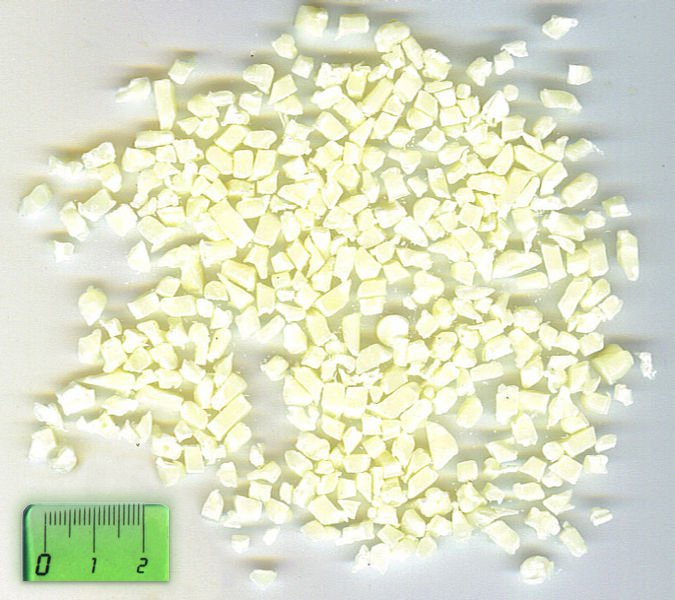
\includegraphics[]{referenzen/Grãos_de_plástico_ABS_(ABS_plastic_grains).jpg}%
            }
            \caption[Unpigmentiertes, Naturfarbenes ABS-Granulat]{Unpigmentiertes, Naturfarbenes ABS-Granulat.}%
            \label{fig:virgin ABS}%
        \end{wrapfigure}
        Eine weiter entwickelte Form des ABS stellt das Acrylnitril-Styrol-Acrylat (ASA) dar. Während die mechanischen und
        thermischen Eigenschaften nahezu identisch bleiben verleiht der Tausch des 1,3-Butadien gegen ein Acrylsäureester
        dem Material eine deutlich höhere UV-Beständigkeit. Aus ASA gefertigte Teile, die häufig dem Sonnenlicht ausgesetzt
        werden, benötigen keine Schutzlackierung mehr. Auch die Produktion ist weitestgehend identisch. Es zeichnet sich
        bereits ein Anstieg der Nachfrage ab was die Vermutung zulässt, dass ASA dem ABS mittelfristig den Rang ablaufen wird.
        Aufgrund des hohen Butadienanteils ist es nicht möglich, ABS völlig transparent Herzustellen. Unpigmentiertes ABS
        ist gelblich bis weiß und leicht transluzent. Es lässt sich allerdings leicht einfärben was insbesondere im Bereich
        des Produktdesigns von Vorteil ist.\par

        Dem in \cref{sec:anwendung} angesprochenen Nachteil des relativ hohen Längenausdehnungskoeffizienten wird durch

        Als Flammhemmende Additive sind organische Halogenide und Antimonoxid zu nennen.